\documentclass[10pt,letterpaper]{article}
\usepackage[margin=1in,hmargin=1in]{geometry}
\usepackage{amsmath}
\usepackage{tikz,url}
\usepackage{amssymb}
\usepackage{fancyhdr}
\usetikzlibrary{matrix}
\usepackage{listings}
\usepackage{tabularx}
\usepackage{xcolor}
\usepackage{graphicx}
\usepackage{graphics}
\usepackage{titling}
\pagestyle{fancy}
\usepackage{float}
\usepackage{fancyvrb}
\usepackage{verbatim}
\usepackage{enumitem}
%\usepackage{float}
%\restylefloat{table}

\fancyhead[LO]{STAT W4201 Advanced Data Analysis}
\fancyhead[RO]{HW 5}
\fancyhead[LE]{STAT W4201 Advanced Data Analysis}
\fancyhead[RE]{HW 5}
\title{\textbf {Homework 5}}
\author{{Qianbo Wang}\\{uni: qw2180}}
\date{}
\setlength{\droptitle}{-5em}
\setlength{\parindent}{0pt}
\makeatletter
\newcommand{\rmnum}[1]{\romannumeral #1}
\newcommand{\Rmnum}[1]{\expandafter\@slowromancap\romannumeral #1@}
\makeatother
\lstset{
language=R,
tabsize=4, 
%frame=shadowbox, 
commentstyle=\color{red!50!green!50!blue!50},
%rulesepcolor=\color{red!20!green!20!blue!20},
keywordstyle=\color{blue!90},
showstringspaces=false,
stringstyle=\ttfamily, 
keepspaces=true, 
breakindent=22pt, 
numbers=none,
stepnumber=1,
numberstyle=\tiny, 
numberstyle={\color[RGB]{0,192,192}\tiny} ,
numbersep=5pt,  
basicstyle=\footnotesize, 
showspaces=false, 
flexiblecolumns=true, 
comment=[l]{\#},
texcl=true,
escapeinside={\$$}{\^^M},
breaklines=true, 
breakautoindent=true,
breakindent=4em, 
aboveskip=1em, 
tabsize=2,
showstringspaces=false, 
backgroundcolor=\color[RGB]{244,244,244},   
fontadjust,
captionpos=t,
framextopmargin=2pt,framexbottommargin=2pt,abovecaptionskip=-3pt,belowcaptionskip=3pt,
extendedchars=false,columns=flexible
}


\begin{document}
\maketitle
\thispagestyle{fancy}
\vspace{-2em}

\large{\textbf{Consider the Boston dataset, in R library MASS, on Housing Values in Suburbs of Boston, to fit a suitable model to predict medv (median value of owner-occupied homes in \$1000s) using the following set of predictors: crim, zn, indus, nox, rm, age, tax.}}\\
\section*{Problem 1}
\textbf{Investigate whether there is any multicollinearity, and suggest remedial measures if appropriate.}\\
\begin{enumerate}[leftmargin=0cm,itemindent=.5cm,labelwidth=\itemindent,labelsep=0cm,align=left]
\item[\textbullet] Detect multicollinearity

I just fit a multilinear regression on the data and then detect the multicollinearity.\\
First, use Variance Inflation Factor to detect if there is multicollinearity among the variables. And the VIFs are as follows:
\begin{center}
ANOVA with VIF Result
\verbatiminput{anova.txt}
\end{center} 

Since from the result we can find that the VIFs of the variables are all $<10$. Then calculate the mean of the $VIF$, $\overline{VIF} = 1.103626>1$. 
Since all $VIF<10$, but the  $\overline{VIF}>1$, i.e. Average Variance of Inflation Factor is larger than 1. So there exists slight multicollinearity.\\

Second, use Condition Number to detect multicollinearity. The Condition Number of the correlation matrix is $19.45283<30$. So we can conclude that there is no serious multicollinearity among the explanatory variables. But there may exist slight multicollinearity. 

\item[\textbullet] Multicollinearity Remedies

1. Use Ridge Regression \\
2. Do transformation on X and Y to get uncorrelated centered data for regression. \\
3. Use Principle Component Regression method to eliminate multicollinearity.
\end{enumerate}

\section*{Problem 2}
\textbf{Compare models selected using LASSO and a stepwise procedure.}\\
\begin{enumerate}[leftmargin=0cm,itemindent=.5cm,labelwidth=\itemindent,labelsep=0cm,align=left]
\item[\textbullet] Lasso Regression

Use Lasso regression with cross validation to choose the best parameter $\lambda$, then we choose the best $\lambda$ as \[\lambda_{opt} =0.0349\] Then get the coefficients of lasso regression, the result is: 
\[medv = -19.46 - 0.1303crim +  0.0213zn - 0.0157indus +  7.5757rm - 0.0228age - 0.0089tax\] 
And the plot is as follows:
\begin{center}
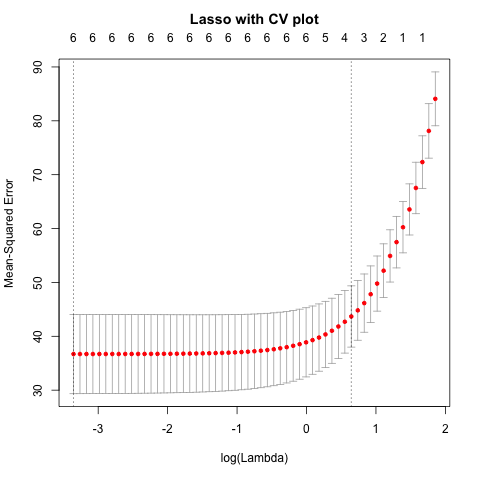
\includegraphics[scale=0.8]{lasso}
\end{center}
And then calculate the mean square error of Lasso regression, $MSE = 35.30283$.\\

\item[\textbullet] Stepwise Regression

Use stepwise regression and use AIC as the parameter to help choose the model.
The forward stepwise regression result is as follows:
\[medv = -19.7132 - 0.1319crim +  0.0229zn  +  7.6253rm - 0.0241age - 0.0093tax\] 
\begin{center}
Forward Stepwise Result
\verbatiminput{forward.txt}
\end{center} 
And the backward stepwise regression result is as follows:
\[medv = -19.7132 - 0.1319crim +  0.0229zn  +  7.6253rm - 0.0241age - 0.0093tax\] 
\begin{center}
Backward Stepwise Result
\verbatiminput{backward.txt}
\end{center} 
Since both forward and backward stepwise regression give the same result, i.e. included crim, zn, tax, age and rm as explanatory variables. Then we should choose this as the stepwise result model.
And then calculate the mean square error of stepwise regression, $MSE = 35.30361$.

\item[\textbullet] Compare 

Compare the two methods, we can find that they have close MSE, but the stepwise model only have 5 explanatory variables, but the lasso contains all explanatory variables.  And since lasso is more complex, so there may exist overfitting in lasso regression. 
\end{enumerate}

\newpage
\textbf{R Code:}
\begin{lstlisting}
rm(list=ls())
library(MASS)
multilinear<-lm(medv~crim+zn+indus+nox+rm+age+tax,data=Boston)
summary(multilinear)

sink("/Users/Qianbo/Google Drive/STAT W4201/HW5/multilinear.txt")
summary(multilinear)
sink()

#VIF detect multicollinearity
anova_table<-anova(multilinear)
SS<-anova(multilinear)$"Sum Sq"
VIF<-1/(1-SS[-length(SS)]/sum(SS))
anova_table$"VIF"<-c(VIF,"")
sink("/Users/Qianbo/Google Drive/STAT W4201/HW5/anova.txt")
anova_table
sink()
VIF_bar<-mean(VIF)

#correlation matrix

names<-c("crim","zn","indus","nox","rm","age","tax")
explanatory<-as.matrix(Boston[names])
dependent<-as.matrix(Boston["medv"])
corr_mat<-cor(explanatory)
eigen_values<-eigen(corr_mat)$values
con_number<-max(eigen_values)/min(eigen_values)

#ridge regression
ridge_reg<-lm.ridge(medv~crim+zn+indus+nox+rm+age+tax,data=Boston)
ridge_coef<-ridge_reg$coef

#Lasso regression
library(glmnet)
names<-c("crim","zn","indus","nox","rm","age","tax")
explanatory<-as.matrix(Boston[names])
dependent<-as.matrix(Boston["medv"])

lasso_reg<-glmnet(explanatory,dependent)
cv_reg<-cv.glmnet(explanatory,dependent)
plot(cv_reg)

png(file="/Users/Qianbo/Google Drive/STAT W4201/HW5/lasso.png")
plot(cv_reg)
title("Lasso with CV plot",line = 2.5)
dev.off()

#choose model coefficient
lambda<-cv_reg$lambda.min
coeff<-coef(cv_reg,s="lambda.min")
predict_lasso<-predict(cv_reg,newx = explanatory,s="lambda.min")
MSE_lasso<-mean((dependent-predict_lasso)^2)

#stepwise regression
glm_model1<-glm(medv~1,data=Boston)
glm_model2<-glm(medv~crim+zn+indus+nox+rm+age+tax,data=Boston)

backward<-stepAIC(glm_model2,direction = "backward",scope=list(
  upper = glm_model2,lower = glm_model1),trace = F)

forward<-stepAIC(glm_model1,direction = "forward",scope=list(
  upper = glm_model2,lower = glm_model1),trace = F)

sink("/Users/Qianbo/Google Drive/STAT W4201/HW5/forward.txt")
forward
sink()
sink("/Users/Qianbo/Google Drive/STAT W4201/HW5/backward.txt")
backward
sink()

#calculate MSE
predict_back<-predict(backward,newx = explanatory)
predict_for<-predict(forward,newx = explanatory)
MSE_back<-mean((dependent-predict_back)^2)
MSE_for<-mean((dependent-predict_for)^2)
\end{lstlisting}
\end{document}